\documentclass[11pt,a4paper]{article}

\usepackage[utf8]{inputenc}
\usepackage[T1]{fontenc}
\usepackage{amsmath,amssymb,amsfonts}
\usepackage{mathtools}
\usepackage{bm}
\usepackage{booktabs}
\usepackage{hyperref}
\usepackage[margin=1in]{geometry}
\usepackage{enumitem}
\usepackage{tikz}
\usetikzlibrary{calc,arrows.meta,positioning,decorations.markings}
\usepackage{blkarray}
\usepackage{amsthm}

\newtheorem{theorem}{Theorem}[section]

% Notation shortcuts
\newcommand{\dd}{\mathrm{d}}
\newcommand{\half}{\tfrac{1}{2}}
\newcommand{\hodge}{\star}

\title{Particle-in-Cell on an Icosahedral Prismatic Mesh:\\
  Formalism and Algorithms}
\author{Working Document}
\date{\today}

\begin{document}
\maketitle

\begin{abstract}
We present a particle-in-cell (PIC) algorithm on a prismatic mesh formed by
extruding an icosahedral triangulation of the sphere along radial layers. The
formalism is based on discrete exterior calculus (DEC) with tensor-product
Whitney forms on triangular prisms. We develop the framework in three stages:
(1)~the mesh geometry, Whitney forms, and incidence operators that define the
discrete complex; (2)~the Maxwell field solver, including the Galerkin Hodge
star, sparse inverse Hodge for explicit updates, and leapfrog time integration;
and (3)~the charge-conserving current deposition scheme, with a proof that
the discrete continuity equation is satisfied exactly. Throughout, we work in
flat space with Euclidean metric to establish the core algorithm.
\end{abstract}

\tableofcontents

%=============================================================================
\section{Mesh and Discrete Complex}
\label{sec:mesh}
%=============================================================================

%-----------------------------------------------------------------------------
\subsection{Angular mesh: icosahedral subdivision}
%-----------------------------------------------------------------------------

Start with the 20-face icosahedron inscribed in the unit sphere, having 12
vertices, 30 edges, and 20 triangular faces. Apply Class~I aperture-4
subdivision: bisect every edge and project the new vertices onto the unit
sphere, producing 4 sub-triangles per parent triangle. After $L$ levels of
subdivision the angular mesh has
\begin{equation}
  N_\triangle = 20 \times 4^L \text{ triangles}, \qquad
  N_v \approx 10 \times 4^L + 2 \text{ vertices}, \qquad
  N_e \approx 30 \times 4^L \text{ edges}.
\end{equation}
At $L = 6$, the mesh has $81{,}920$ triangles with angular resolution
$\sim 1^\circ$, comparable to a $256 \times 512$ grid in
$(\theta,\varphi)$ but with nearly uniform cell areas and no polar degeneracy.

Spring-dynamics optimization~\cite{Tomita2002} can further equalize cell areas,
reducing the max/min area ratio to $\sim 1.2$.

\paragraph{Computable connectivity.}
Within a single icosahedral base face, subdivision level $L$ produces a
regular triangular lattice indexed by barycentric grid coordinates $(i, j)$
with $0 \le i + j \le 2^L$. The three neighbors of any sub-triangle are
determined by arithmetic on $(i, j)$. Across base-face boundaries, the
adjacency of the 20 icosahedral faces is encoded in a fixed $20 \times 3$
lookup table (60 entries). The full neighbor function is therefore
\emph{computable from the element index}---no connectivity arrays are stored
in memory.

%-----------------------------------------------------------------------------
\subsection{Prismatic cells}
%-----------------------------------------------------------------------------

Define $N_r$ radial shells at radii $r_0 < r_1 < \cdots < r_{N_r}$ (e.g.,
logarithmically spaced). Each angular triangle
$(\hat{\bm{n}}_1, \hat{\bm{n}}_2, \hat{\bm{n}}_3)$ combined with a radial
shell pair $(r_k, r_{k+1})$ defines a triangular prism with 6 vertices at
Cartesian positions
\begin{equation}
  \bm{x}_{i,j} = r_j \, \hat{\bm{n}}_i, \qquad
  i \in \{1,2,3\}, \quad j \in \{k, k+1\}.
\end{equation}
The combinatorial structure is that of a triangular prism: 6 vertices,
9 edges, and 5 faces. The total mesh has $N_\triangle \times N_r$ prisms.
Radial neighbors are $\pm 1$ in the layer index $k$.

%-----------------------------------------------------------------------------
\subsection{Prism geometry and labeling}
\label{sec:labeling}
%-----------------------------------------------------------------------------

We label the elements of a single prism as follows
(Figure~\ref{fig:prism}):

\begin{itemize}[nosep]
  \item \textbf{Vertices} $v_1,\ldots,v_6$: $v_1 = (1,0)$, $v_2 = (2,0)$,
    $v_3 = (3,0)$ on the bottom triangle, and $v_4 = (1,1)$, $v_5 = (2,1)$,
    $v_6 = (3,1)$ on the top.
  \item \textbf{Horizontal edges} (6): $h_1: v_1 \to v_2$,
    $h_2: v_2 \to v_3$, $h_3: v_3 \to v_1$ (bottom); $h_4: v_4 \to v_5$,
    $h_5: v_5 \to v_6$, $h_6: v_6 \to v_4$ (top).
  \item \textbf{Vertical edges} (3): $\ell_1: v_1 \to v_4$,
    $\ell_2: v_2 \to v_5$, $\ell_3: v_3 \to v_6$.
  \item \textbf{Triangular faces}: $f_\bot$ (bottom) and $f_\top$ (top).
  \item \textbf{Rectangular faces} (3): $f_{12}$, $f_{23}$, $f_{31}$, each
    spanned by the two endpoints of the corresponding triangle edge at both
    radial levels.
\end{itemize}

\begin{figure}[ht]
\centering
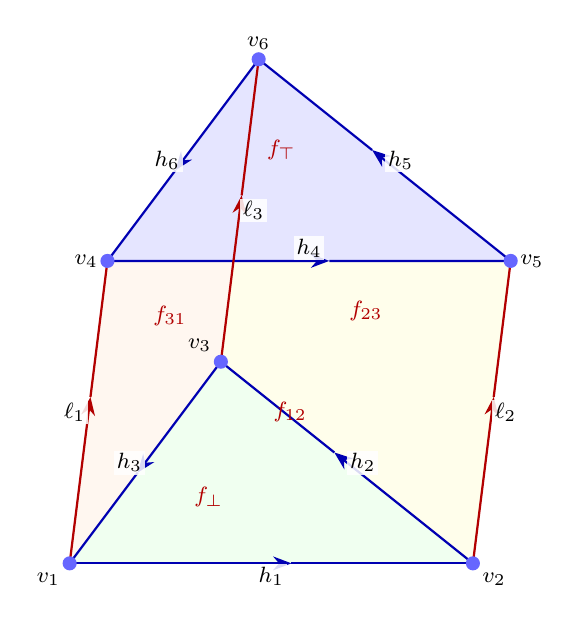
\begin{tikzpicture}[scale=1.6,
    vertex/.style={circle, fill=blue!60, inner sep=1.8pt},
    edge_label/.style={font=\footnotesize, fill=white, inner sep=1pt,
      opacity=0.85, text opacity=1},
    face_label/.style={font=\footnotesize\itshape, text=red!70!black},
    >=Stealth
  ]
  % --- Bottom triangle ---
  \coordinate (A0) at (0, 0);
  \coordinate (B0) at (3.2, 0);
  \coordinate (C0) at (1.2, 1.6);
  % --- Top triangle ---
  \coordinate (A1) at (0.3, 2.4);
  \coordinate (B1) at (3.5, 2.4);
  \coordinate (C1) at (1.5, 4.0);

  % --- Faces (shaded) ---
  \fill[blue!6] (A0) -- (B0) -- (C0) -- cycle;
  \fill[green!6] (A0) -- (B0) -- (B1) -- (A1) -- cycle;
  \fill[orange!6] (C0) -- (A0) -- (A1) -- (C1) -- cycle;
  \fill[yellow!8] (B0) -- (C0) -- (C1) -- (B1) -- cycle;
  \fill[blue!10] (A1) -- (B1) -- (C1) -- cycle;

  % --- Bottom edges ---
  \draw[->, thick, blue!70!black] (A0) -- ($(A0)!0.55!(B0)$);
  \draw[thick, blue!70!black] ($(A0)!0.55!(B0)$) -- (B0);
  \draw[->, thick, blue!70!black] (B0) -- ($(B0)!0.55!(C0)$);
  \draw[thick, blue!70!black] ($(B0)!0.55!(C0)$) -- (C0);
  \draw[->, thick, blue!70!black] (C0) -- ($(C0)!0.55!(A0)$);
  \draw[thick, blue!70!black] ($(C0)!0.55!(A0)$) -- (A0);

  % --- Top edges ---
  \draw[->, thick, blue!70!black] (A1) -- ($(A1)!0.55!(B1)$);
  \draw[thick, blue!70!black] ($(A1)!0.55!(B1)$) -- (B1);
  \draw[->, thick, blue!70!black] (B1) -- ($(B1)!0.55!(C1)$);
  \draw[thick, blue!70!black] ($(B1)!0.55!(C1)$) -- (C1);
  \draw[->, thick, blue!70!black] (C1) -- ($(C1)!0.55!(A1)$);
  \draw[thick, blue!70!black] ($(C1)!0.55!(A1)$) -- (A1);

  % --- Vertical edges ---
  \draw[->, thick, red!70!black] (A0) -- ($(A0)!0.55!(A1)$);
  \draw[thick, red!70!black] ($(A0)!0.55!(A1)$) -- (A1);
  \draw[->, thick, red!70!black] (B0) -- ($(B0)!0.55!(B1)$);
  \draw[thick, red!70!black] ($(B0)!0.55!(B1)$) -- (B1);
  \draw[->, thick, red!70!black] (C0) -- ($(C0)!0.55!(C1)$);
  \draw[thick, red!70!black] ($(C0)!0.55!(C1)$) -- (C1);

  % --- Vertices ---
  \node[vertex] at (A0) {};
  \node[vertex] at (B0) {};
  \node[vertex] at (C0) {};
  \node[vertex] at (A1) {};
  \node[vertex] at (B1) {};
  \node[vertex] at (C1) {};

  % --- Vertex labels ---
  \node[below left, font=\footnotesize] at (A0) {$v_1$};
  \node[below right, font=\footnotesize] at (B0) {$v_2$};
  \node[above left, font=\footnotesize] at (C0) {$v_3$};
  \node[left, font=\footnotesize] at (A1) {$v_4$};
  \node[right, font=\footnotesize] at (B1) {$v_5$};
  \node[above, font=\footnotesize] at (C1) {$v_6$};

  % --- Edge labels ---
  \node[edge_label, below] at ($(A0)!0.5!(B0)$) {$h_1$};
  \node[edge_label, right] at ($(B0)!0.5!(C0)$) {$h_2$};
  \node[edge_label, left] at ($(C0)!0.5!(A0)$) {$h_3$};
  \node[edge_label, above] at ($(A1)!0.5!(B1)$) {$h_4$};
  \node[edge_label, right] at ($(B1)!0.5!(C1)$) {$h_5$};
  \node[edge_label, left] at ($(C1)!0.5!(A1)$) {$h_6$};
  \node[edge_label, left] at ($(A0)!0.5!(A1)$) {$\ell_1$};
  \node[edge_label, right] at ($(B0)!0.5!(B1)$) {$\ell_2$};
  \node[edge_label, right] at ($(C0)!0.5!(C1)$) {$\ell_3$};

  % --- Face labels ---
  \node[face_label] at ($(A0)!0.33!(B0)!0.33!(C0)$) {$f_\bot$};
  \node[face_label] at ($(A1)!0.5!(B1)!0.55!(C1)$) {$f_\top$};
  \node[face_label] at ($(A0)!0.5!(B1)$) {$f_{12}$};
  \node[face_label] at ($(B0)!0.5!(C1)$) {$f_{23}$};
  \node[face_label] at ($(C0)!0.45!(A1)$) {$f_{31}$};
\end{tikzpicture}
\caption{A single prismatic cell with labeled vertices ($v_1,\ldots,v_6$),
  horizontal edges ($h_1,\ldots,h_6$, blue), vertical edges
  ($\ell_1,\ell_2,\ell_3$, red), and faces ($f_\bot, f_\top, f_{12}, f_{23},
  f_{31}$). Arrows indicate the chosen edge orientations.}
\label{fig:prism}
\end{figure}

%-----------------------------------------------------------------------------
\subsection{Coordinates on the prism}
\label{sec:coordinates}
%-----------------------------------------------------------------------------

The prism is the product of a triangle $T$ and a radial interval $I$.
We introduce two sets of coordinates:

\paragraph{Barycentric coordinates.}
Let $(\lambda_1, \lambda_2, \lambda_3)$ be the barycentric coordinates on
triangle $T$, defined by $\lambda_i \geq 0$ and
$\lambda_1 + \lambda_2 + \lambda_3 = 1$. Any point in $T$ can be written as
$\bm{x}_T = \lambda_1 \bm{x}_1 + \lambda_2 \bm{x}_2 + \lambda_3 \bm{x}_3$,
where $\bm{x}_i$ are the triangle vertices. Given an arbitrary point $\bm{x}_T$
in the plane of the triangle, the barycentric coordinates are computed by
solving a $2\times 2$ linear system.

\paragraph{Radial coordinate.}
Let $\zeta \in [0,1]$ parameterize the radial interval, with $\zeta = 0$
at the bottom level ($r_k$) and $\zeta = 1$ at the top ($r_{k+1}$). We define
the radial hat functions:
\begin{equation}
  \varphi_0(\zeta) = 1 - \zeta, \qquad \varphi_1(\zeta) = \zeta.
  \label{eq:hat_functions}
\end{equation}
These satisfy $\varphi_0 + \varphi_1 = 1$.

A point inside the prism is fully specified by $(\lambda_1, \lambda_2,
\lambda_3, \zeta)$, subject to $\sum_i \lambda_i = 1$, $\lambda_i \geq 0$,
and $0 \leq \zeta \leq 1$.

%-----------------------------------------------------------------------------
\subsection{Whitney forms}
\label{sec:whitney}
%-----------------------------------------------------------------------------

The tensor-product Whitney forms provide a basis for interpolating discrete
cochains (values at vertices, edges, faces) into continuous differential forms
on the prism interior. They are constructed as products of the 2D Whitney forms
on triangle $T$ and the 1D hat functions on interval $I$.

\paragraph{0-forms (6 per prism, one per vertex).}
\begin{equation}
  W^0_{i,j}(\lambda, \zeta) = \lambda_i \, \varphi_j(\zeta), \qquad
  i \in \{1,2,3\},\; j \in \{0,1\}.
  \label{eq:W0}
\end{equation}
These form a partition of unity:
$\sum_{i,j} W^0_{i,j} = (\sum_i \lambda_i)(\sum_j \varphi_j) = 1$.
Each $W^0_{i,j}$ equals 1 at vertex $v_{i,j}$ and 0 at all other vertices.

\paragraph{1-forms (9 per prism, one per edge).}
The 6 horizontal edge forms and 3 vertical edge forms are:
\begin{align}
  W^1_{ij,k} &= (\lambda_i \, \dd\lambda_j - \lambda_j \, \dd\lambda_i)
    \,\varphi_k(\zeta)
  && \text{(horizontal edge from $v_i$ to $v_j$ at level $k$)},
  \label{eq:W1h} \\
  W^1_i &= \lambda_i \, \dd\zeta
  && \text{(vertical edge at triangle vertex $i$)}.
  \label{eq:W1v}
\end{align}

\paragraph{2-forms (5 per prism, one per face).}
\begin{align}
  W^2_k &= 2\,\dd\lambda_1 \wedge \dd\lambda_2 \;\varphi_k(\zeta)
  && \text{(triangular face at level $k$)},
  \label{eq:W2tri} \\
  W^2_{ij} &= (\lambda_i \, \dd\lambda_j - \lambda_j \, \dd\lambda_i)
    \wedge \dd\zeta
  && \text{(rectangular face on edge $ij$)}.
  \label{eq:W2rect}
\end{align}

\paragraph{3-form (1 per prism).}
\begin{equation}
  W^3 = 2\,\dd\lambda_1 \wedge \dd\lambda_2 \wedge \dd\zeta.
  \label{eq:W3}
\end{equation}

%-----------------------------------------------------------------------------
\subsection{Incidence matrices}
\label{sec:incidence}
%-----------------------------------------------------------------------------

The incidence matrices encode the combinatorial boundary structure of the
complex. They are purely topological---independent of vertex positions or
metric.

\paragraph{Gradient operator $\dd_0$ ($9\times 6$, edges $\times$ vertices).}
The entry $(\dd_0)_{ev}$ is $+1$ if $v$ is the head of edge $e$, $-1$ if
$v$ is the tail, and $0$ otherwise:
\begin{equation}
  \dd_0 =
  \begin{blockarray}{ccccccc}
    & v_1 & v_2 & v_3 & v_4 & v_5 & v_6 \\
    \begin{block}{c(cccccc)}
      h_1 & -1 & +1 &  0 &  0 &  0 &  0 \\
      h_2 &  0 & -1 & +1 &  0 &  0 &  0 \\
      h_3 & +1 &  0 & -1 &  0 &  0 &  0 \\
      h_4 &  0 &  0 &  0 & -1 & +1 &  0 \\
      h_5 &  0 &  0 &  0 &  0 & -1 & +1 \\
      h_6 &  0 &  0 &  0 & +1 &  0 & -1 \\
      \ell_1 & -1 &  0 &  0 & +1 &  0 &  0 \\
      \ell_2 &  0 & -1 &  0 &  0 & +1 &  0 \\
      \ell_3 &  0 &  0 & -1 &  0 &  0 & +1 \\
    \end{block}
  \end{blockarray}
  \label{eq:d0}
\end{equation}

\paragraph{Curl operator $\dd_1$ ($5\times 9$, faces $\times$ edges).}
The entry $(\dd_1)_{fe}$ is $+1$ ($-1$) if edge $e$ appears with positive
(negative) orientation in the boundary of face $f$:
\begin{equation}
  \dd_1 =
  \begin{blockarray}{cccccccccc}
    & h_1 & h_2 & h_3 & h_4 & h_5 & h_6 & \ell_1 & \ell_2 & \ell_3 \\
    \begin{block}{c(ccccccccc)}
      f_\bot & -1 & -1 & -1 & 0 & 0 & 0 & 0 & 0 & 0 \\
      f_\top & 0 & 0 & 0 & +1 & +1 & +1 & 0 & 0 & 0 \\
      f_{12} & +1 & 0 & 0 & -1 & 0 & 0 & -1 & +1 & 0 \\
      f_{23} & 0 & +1 & 0 & 0 & -1 & 0 & 0 & -1 & +1 \\
      f_{31} & 0 & 0 & +1 & 0 & 0 & -1 & +1 & 0 & -1 \\
    \end{block}
  \end{blockarray}
  \label{eq:d1}
\end{equation}

These matrices satisfy the fundamental identity
\begin{equation}
  \dd_1 \cdot \dd_0 = 0,
  \label{eq:dd_zero}
\end{equation}
which is the discrete statement that ``the boundary of a boundary is zero.''
This is verified row by row; for example, row $f_{12}$ applied to $v_1$:
$(+1)(-1) + (-1)(0) + (-1)(-1) + (+1)(0) = 0$.

%-----------------------------------------------------------------------------
\subsection{The Whitney commuting property}
\label{sec:commuting}
%-----------------------------------------------------------------------------

The central algebraic identity relating the continuous and discrete structures
is
\begin{equation}
  \boxed{
    \dd W^0_v = \sum_e (\dd_0)_{e,v}\;W^1_e
    \qquad \text{for every vertex } v,
  }
  \label{eq:commuting}
\end{equation}
i.e., the exterior derivative of each Whitney 0-form equals the corresponding
linear combination of Whitney 1-forms, with coefficients given by the incidence
matrix. This property is the bridge between continuous calculus (the exterior
derivative $\dd$) and discrete topology (the matrix $\dd_0$).

\begin{proof}[Verification for $v_1 = (1,0)$]
By the product rule:
\begin{equation}
  \dd W^0_{1,0} = \dd(\lambda_1 \varphi_0)
    = (\dd\lambda_1)\,\varphi_0 + \lambda_1\,(\dd\varphi_0)
    = (\dd\lambda_1)\,\varphi_0 - \lambda_1\,\dd\zeta.
  \label{eq:dW0_expanded}
\end{equation}

\emph{Vertical part.} The second term is $-\lambda_1\,\dd\zeta = -W^1_1$.
Since $(\dd_0)_{\ell_1, v_1} = -1$, the contribution is
$(-1)\cdot W^1_1 = -W^1_1$. \checkmark

\emph{Horizontal part.} The edges incident to $v_1$ at level 0 are $h_1$
(tail, coefficient $-1$) and $h_3$ (head, coefficient $+1$). The sum:
\begin{align}
  (-1)\,W^1_{12,0} + (+1)\,W^1_{31,0}
  &= -(\lambda_1\,\dd\lambda_2 - \lambda_2\,\dd\lambda_1)\,\varphi_0
    + (\lambda_3\,\dd\lambda_1 - \lambda_1\,\dd\lambda_3)\,\varphi_0 \notag\\
  &= \bigl[(\lambda_2 + \lambda_3)\,\dd\lambda_1
    - \lambda_1(\dd\lambda_2 + \dd\lambda_3)\bigr]\,\varphi_0.
\end{align}
Using $\lambda_2 + \lambda_3 = 1 - \lambda_1$ and
$\dd\lambda_2 + \dd\lambda_3 = -\dd\lambda_1$:
\begin{equation}
  = \bigl[(1 - \lambda_1) + \lambda_1\bigr]\,\dd\lambda_1\,\varphi_0
  = (\dd\lambda_1)\,\varphi_0. \quad\checkmark
\end{equation}
Combining both parts reproduces~\eqref{eq:dW0_expanded}. The proof for all
other vertices follows by permuting indices and exchanging radial levels.
\end{proof}

%=============================================================================
\section{Maxwell Field Solver}
\label{sec:maxwell}
%=============================================================================

%-----------------------------------------------------------------------------
\subsection{Degrees of freedom}
\label{sec:dof}
%-----------------------------------------------------------------------------

The electromagnetic degrees of freedom are assigned to geometric elements of
the primal complex:

\begin{center}
\begin{tabular}{llll}
  \toprule
  Quantity & Element & Count/prism & Meaning \\
  \midrule
  $\rho_v$ (charge density) & vertex $v$ & 6
    & charge in dual volume around $v$ \\
  $D_e$ (electric flux) & edge $e$ & 9
    & $\int_e \bm{D}\cdot\dd\bm{\ell}$ \\
  $B_f$ (magnetic flux) & face $f$ & 5
    & $\int_f \bm{B}\cdot\dd\bm{S}$ \\
  $J_e$ (current) & edge $e$ & 9
    & $\int_e \bm{J}\cdot\dd\bm{\ell}$ \\
  \bottomrule
\end{tabular}
\end{center}

The field solver computes auxiliary fields $\widetilde{E}_e$ and
$\widetilde{H}_f$ from $D_e$ and $B_f$ through constitutive relations (the
Hodge star), and uses them in the update equations.

%-----------------------------------------------------------------------------
\subsection{Update equations}
\label{sec:update_eqs}
%-----------------------------------------------------------------------------

Faraday's law and Amp\`ere's law take the compact form:
\begin{align}
  \frac{\partial B_f}{\partial t}
    &= -\sum_e (\dd_1)_{fe}\;\widetilde{E}_e,
    \label{eq:faraday} \\
  \frac{\partial D_e}{\partial t}
    &= +\sum_f (\dd_1^T)_{ef}\;\widetilde{H}_f - J_e.
    \label{eq:ampere}
\end{align}
Faraday's law~\eqref{eq:faraday} uses the curl matrix $\dd_1$
from~\eqref{eq:d1}: the change in magnetic flux through face $f$ is the
(signed) circulation of the auxiliary electric field around the boundary of $f$.
Amp\`ere's law~\eqref{eq:ampere} uses $\dd_1^T$: the change in electric
flux along edge $e$ is driven by the auxiliary magnetic field on the faces
incident to $e$, minus the deposited current.

\paragraph{Structural conservation laws.}
The identity $\dd_1 \cdot \dd_0 = 0$ implies two exact conservation laws:
\begin{enumerate}[nosep]
  \item \emph{Divergence-free $B$.} Let $\dd_2$ be the face-to-volume incidence
    matrix. Then $\dd_2 \cdot \dd_1 = 0$, so
    $\partial_t (\dd_2 B) = -\dd_2 \dd_1 \widetilde{E} = 0$: the discrete
    divergence of $B$ is exactly preserved.
  \item \emph{Charge continuity.} Taking $\dd_0^T$ of
    Amp\`ere's law and using
    $\dd_0^T \dd_1^T = (\dd_1 \dd_0)^T = 0$:
    \begin{equation}
      \frac{\partial}{\partial t}\bigl(\dd_0^T D\bigr)_v
        = -(\dd_0^T J)_v.
      \label{eq:discrete_continuity}
    \end{equation}
    The rate of change of charge at vertex $v$ equals the net current flowing
    into $v$.
\end{enumerate}
Both identities are exact (to machine precision) and hold regardless of the
constitutive relations.

\paragraph{Expanded Faraday update.}
Using the incidence matrix~\eqref{eq:d1}, the five face updates are:
\begin{align}
  \partial_t B_{f_\bot}
    &= +\widetilde{E}_{h_1} + \widetilde{E}_{h_2}
      + \widetilde{E}_{h_3}, \nonumber\\
  \partial_t B_{f_\top}
    &= -\widetilde{E}_{h_4} - \widetilde{E}_{h_5}
      - \widetilde{E}_{h_6}, \nonumber\\
  \partial_t B_{f_{12}}
    &= -\widetilde{E}_{h_1} + \widetilde{E}_{h_4}
      + \widetilde{E}_{\ell_1} - \widetilde{E}_{\ell_2}, \nonumber\\
  \partial_t B_{f_{23}}
    &= -\widetilde{E}_{h_2} + \widetilde{E}_{h_5}
      + \widetilde{E}_{\ell_2} - \widetilde{E}_{\ell_3}, \nonumber\\
  \partial_t B_{f_{31}}
    &= -\widetilde{E}_{h_3} + \widetilde{E}_{h_6}
      - \widetilde{E}_{\ell_1} + \widetilde{E}_{\ell_3}.
  \label{eq:faraday_expanded}
\end{align}

\paragraph{Expanded Amp\`ere update (examples).}
Reading columns of $\dd_1$, the updates for $h_1$ and $\ell_1$ are:
\begin{align}
  \partial_t D_{h_1} &= -\widetilde{H}_{f_\bot}
    + \widetilde{H}_{f_{12}} - J_{h_1}, \\
  \partial_t D_{\ell_1} &= -\widetilde{H}_{f_{12}}
    + \widetilde{H}_{f_{31}} - J_{\ell_1}.
\end{align}

%-----------------------------------------------------------------------------
\subsection{Constitutive relations: the circumcentric dual Hodge}
\label{sec:hodge}
%-----------------------------------------------------------------------------

The update equations~\eqref{eq:faraday}--\eqref{eq:ampere} require computing
auxiliary fields $\widetilde{E}$ and $\widetilde{H}$ from the primary fields
$E$ and $B$. In flat space, $\bm{E} = \bm{D}$ and $\bm{H} = \bm{B}$ as
continuous vector fields, but the discrete edge integral $E_e = \int_e
\bm{E}\cdot\dd\bm{\ell}$ and the dual face integral $D_{e^*} = \int_{e^*}
\bm{D}\cdot\dd\bm{S}$ are integrals over different geometric objects. The
Hodge star maps between them.

The integral form of Maxwell's equations is exact on the discrete complex:
Faraday computes the circulation of $E$ around each primal face, and Amp\`ere
computes the circulation of $H$ around each dual face. Both are purely
topological operations involving only the incidence matrices $\dd_1$ and
$\dd_1^T$. The \emph{only} approximation enters in the constitutive
relations that convert between primal and dual quantities.

\paragraph{Circumcentric (Voronoi) dual.}
For each prism in the mesh, a dual vertex is placed at the \emph{circumcenter}:
the circumcenter of the angular triangle (equidistant from all three vertices)
at the radial midpoint of the layer. The dual face of a primal edge $e$ is
the polygon formed by connecting the dual vertices (circumcenters) of all
prisms sharing that edge. The dual edge of a primal face $f$ connects the
dual vertices of the two prisms sharing $f$.

The diagonal Hodge star is then:
\begin{equation}
  \hodge_1^{-1}[e] = \frac{|e|}{|e^*|}, \qquad
  \hodge_2[f] = \frac{|f^*|}{|f|},
  \label{eq:circumcentric_hodge}
\end{equation}
where $|e^*|$ is the area of the dual face and $|f^*|$ is the length of the
dual edge. By construction, the circumcentric dual face of each edge is
\emph{perpendicular} to the edge, which is the key property ensuring that
the diagonal Hodge is consistent.

\paragraph{Why circumcenters, not centroids.}
On a non-orthogonal mesh such as the icosahedral triangulation, the diagonal
Hodge assumes that the field component along a primal edge equals the field
component through the dual face. This is exact when the edge is perpendicular
to the dual face, which holds for the circumcentric dual (Voronoi construction)
but not for a centroid-based dual. Empirically, using centroids instead of
circumcenters leads to $\sim 20$--$60\%$ energy drift in a static field test,
while circumcenters reduce this to $\sim 2$--$3\%$.

\paragraph{Computation of dual face areas.}
The dual face of a \emph{horizontal edge} (on a radial shell) is a
quadrilateral formed by the circumcenters of the 4 prisms sharing that edge
(2 angular neighbors $\times$ 2 radial layers). For boundary edges on the
innermost or outermost shell, only 2 prisms contribute; the area is estimated
by mirroring.

The dual face of a \emph{vertical edge} (between radial shells) is a pentagon
or hexagon formed by the circumcenters of the 5--6 prisms surrounding the
vertex at that layer. The polygon area is computed by fan triangulation: the
polygon is decomposed into triangles from the edge midpoint to each pair of
adjacent circumcenters, and the individual triangle areas are summed.

\paragraph{Computation of dual edge lengths.}
The dual edge of a \emph{triangular face} (on a radial shell) connects the
circumcenters of the two prisms above and below. Its length is simply the
Euclidean distance between the two circumcenters.

The dual edge of a \emph{rectangular face} (between radial shells) connects
the circumcenters of the two angularly adjacent prisms. Its length is again
the Euclidean distance.

\paragraph{Galerkin formulation and the mass-matrix-free update.}
In the Galerkin weak form of Maxwell's equations, the mass matrix $M_2$
cancels in Faraday's law (the same $M_2$ appears on both sides), giving an
exact topological update:
\begin{equation}
  \frac{\partial B_f}{\partial t} = -\sum_e (\dd_1)_{fe}\;E_e.
  \label{eq:faraday_exact}
\end{equation}
No Hodge star is needed for Faraday. The Hodge enters only in Amp\`ere's law:
\begin{equation}
  \frac{\partial E_e}{\partial t}
    = \hodge_1^{-1}[e]\;\sum_f (\dd_1^T)_{ef}\;\hodge_2[f]\;B_f - J_e.
  \label{eq:ampere_hodge}
\end{equation}
Since $\hodge_1^{-1}$ and $\hodge_2$ are diagonal, this is a fully explicit
update requiring only one pass over the edges, with no matrix solve.

%-----------------------------------------------------------------------------
\subsection{Leapfrog time integration}
\label{sec:leapfrog}
%-----------------------------------------------------------------------------

We use standard leapfrog (Yee-type) time staggering: $B$ is defined at
half-integer timesteps $t^{n+1/2}$ and $E$ at integer timesteps $t^n$
(Figure~\ref{fig:leapfrog}).

\begin{figure}[ht]
\centering
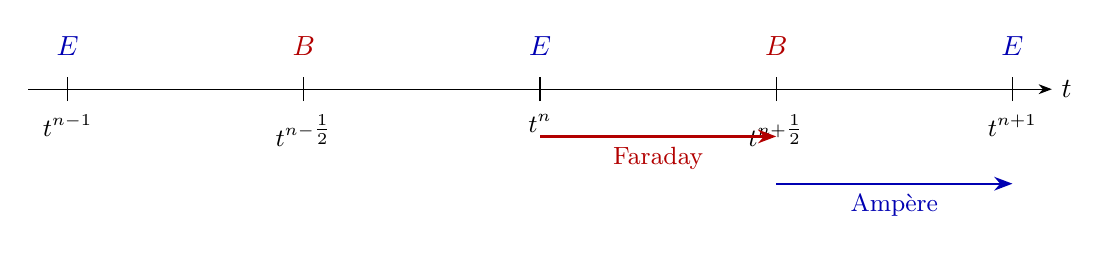
\begin{tikzpicture}[>=Stealth, scale=1.0]
  % Time axis
  \draw[->] (-0.5, 0) -- (12.5, 0) node[right] {$t$};

  % Tick marks
  \foreach \x/\lab in {0/{n-1}, 3/{n-\half}, 6/{n}, 9/{n+\half}, 12/{n+1}} {
    \draw (\x, -0.15) -- (\x, 0.15);
    \node[below] at (\x, -0.2) {\small $t^{\lab}$};
  }

  % E at integer steps
  \foreach \x in {0, 6, 12} {
    \node[above, blue!70!black, font=\bfseries] at (\x, 0.3) {$E$};
  }

  % B at half-integer steps
  \foreach \x in {3, 9} {
    \node[above, red!70!black, font=\bfseries] at (\x, 0.3) {$B$};
  }

  % Update arrows
  \draw[->, thick, red!70!black] (6, -0.6) -- (9, -0.6)
    node[midway, below, font=\small] {Faraday};
  \draw[->, thick, blue!70!black] (9, -1.2) -- (12, -1.2)
    node[midway, below, font=\small] {Amp\`ere};
\end{tikzpicture}
\caption{Leapfrog time staggering. $E$ is defined at integer steps; $B$ at
  half-integer steps. Faraday's law advances $B$ using $E$ directly (no Hodge
  needed). Amp\`ere's law advances $E$ using $\hodge_1^{-1}$ and $\hodge_2$
  applied to $B$.}
\label{fig:leapfrog}
\end{figure}

A full update cycle from $t^n$ to $t^{n+1}$ consists of two steps:
\begin{enumerate}
  \item \textbf{Faraday: $B^{n-1/2} \to B^{n+1/2}$ (exact, no Hodge).}
    \begin{equation}
      B_f^{n+1/2} = B_f^{n-1/2}
        - \Delta t \sum_e (\dd_1)_{fe}\,E_e^n.
    \end{equation}
    This is a purely topological operation: the change in magnetic flux
    through face $f$ equals the circulation of $E$ around the face boundary.
    No constitutive relation is needed because the Galerkin mass matrix
    $M_2$ cancels on both sides.

  \item \textbf{Amp\`ere: $E^n \to E^{n+1}$ (diagonal Hodge).}
    \begin{equation}
      E_e^{n+1} = E_e^n + \Delta t\;\hodge_1^{-1}[e]\;\sum_f
        (\dd_1^T)_{ef}\;\hodge_2[f]\;B_f^{n+1/2}
        - \Delta t\,J_e^{n+1/2}.
    \end{equation}
    This applies the diagonal Hodge star~\eqref{eq:circumcentric_hodge}
    to convert the face-integrated $B$ to a dual-edge quantity, computes
    the dual curl via $\dd_1^T$, and divides by the dual face area via
    $\hodge_1^{-1}$. Since both Hodge factors are diagonal, the entire
    update is a single loop over edges with no matrix solve.
\end{enumerate}

\paragraph{CFL condition.}
The leapfrog scheme is conditionally stable. The maximum timestep is
\begin{equation}
  \Delta t < C_\text{CFL}\;\min_{\text{edges}} |e|,
  \label{eq:cfl}
\end{equation}
where $|e|$ is the primal edge length and $C_\text{CFL}$ is a constant
determined by the stencil geometry. Empirically, for the icosahedral prismatic
mesh with circumcentric dual:
\begin{equation}
  C_\text{CFL} \approx 0.73.
  \label{eq:cfl_number}
\end{equation}
This is comparable to the theoretical leapfrog CFL limit of $1/\sqrt{3}
\approx 0.577$ on a cubic grid, indicating that the circumcentric dual
produces a well-conditioned scheme without artificial wave speed amplification.

With logarithmic radial spacing $r_k = r_\text{min}\,e^{k\Delta x}$, both the
radial edge length $\Delta r_k = r_k \Delta x$ and the angular edge length
$r_k \Delta\theta$ scale as $r_k$. The minimum edge length therefore occurs at
the inner boundary and equals $\min(r_\text{min}\,\Delta x,\;
r_\text{min}\,\Delta\theta)$. The CFL constraint scales as
\begin{equation}
  \Delta t \propto \frac{r_\text{min}}{\max(N_r,\,2^L)},
\end{equation}
which is the standard first-order CFL scaling with resolution --- no artificial
resolution-dependent wave speed amplification occurs with the circumcentric
dual.

\paragraph{Discrete energy.}
The Hodge-weighted discrete electromagnetic energy is
\begin{equation}
  U = \half\sum_e E_e^2\;\hodge_1[e]
    + \half\sum_f B_f^2\;\hodge_2[f],
  \label{eq:discrete_energy}
\end{equation}
where $\hodge_1[e] = |e^*|/|e| = 1/\hodge_1^{-1}[e]$.
The leapfrog scheme with the circumcentric dual conserves this energy to
within $\sim 2$--$3\%$ over long integrations (tested with a static dipole
field over $\sim 10$ light-crossing times).

%=============================================================================
\section{Charge-Conserving Current Deposition}
\label{sec:deposition}
%=============================================================================

%-----------------------------------------------------------------------------
\subsection{Overview}
%-----------------------------------------------------------------------------

When a particle moves from $\bm{x}_\text{old}$ to $\bm{x}_\text{new}$ during
a timestep $\Delta t$, we must deposit current on the 9 edges of the
containing prism such that the discrete continuity
equation~\eqref{eq:discrete_continuity} is satisfied exactly. The key
ingredients are: (i)~the Whitney commuting property~\eqref{eq:commuting},
(ii)~the fundamental theorem of line integrals, and (iii)~the continuity of the
Whitney 0-forms across shared faces for multi-prism trajectories.

%-----------------------------------------------------------------------------
\subsection{Current definition}
\label{sec:current_def}
%-----------------------------------------------------------------------------

The charge of a particle at position $(\lambda, \zeta)$ within a prism is
distributed to the 6 vertices via the Whitney 0-forms~\eqref{eq:W0}:
\begin{equation}
  \rho_v = q\;W^0_v(\bm{x}), \qquad
  \text{so that } \sum_v \rho_v = q.
  \label{eq:charge_deposit}
\end{equation}

The current deposited on edge $e$ is defined as the line integral of the
Whitney 1-form along the particle trajectory $\gamma$:
\begin{equation}
  J_e \equiv \frac{q}{\Delta t} \int_\gamma W^1_e.
  \label{eq:current_def}
\end{equation}

%-----------------------------------------------------------------------------
\subsection{Charge conservation}
\label{sec:conservation}
%-----------------------------------------------------------------------------

\begin{theorem}[Exact charge conservation]
\label{thm:conservation}
With the charge and current definitions~\eqref{eq:charge_deposit}
and~\eqref{eq:current_def}, the discrete continuity equation holds exactly at
every vertex $v$:
\begin{equation}
  \boxed{
    \frac{\Delta\rho_v}{\Delta t} = \sum_e (\dd_0)_{e,v}\;J_e,
  }
  \label{eq:charge_conservation}
\end{equation}
where $\Delta\rho_v = q\bigl[W^0_v(\bm{x}_\text{new}) -
W^0_v(\bm{x}_\text{old})\bigr]$.
\end{theorem}

\begin{proof}
By the fundamental theorem of line integrals:
\begin{equation}
  W^0_v(\bm{x}_\text{new}) - W^0_v(\bm{x}_\text{old})
    = \int_\gamma \dd W^0_v.
\end{equation}
Applying the Whitney commuting property~\eqref{eq:commuting}:
\begin{equation}
  \int_\gamma \dd W^0_v
    = \int_\gamma \sum_e (\dd_0)_{e,v}\;W^1_e
    = \sum_e (\dd_0)_{e,v} \int_\gamma W^1_e.
\end{equation}
Multiplying by $q/\Delta t$ and using
definitions~\eqref{eq:charge_deposit}--\eqref{eq:current_def}:
\begin{equation}
  \frac{\Delta\rho_v}{\Delta t}
    = \frac{q}{\Delta t}\sum_e (\dd_0)_{e,v} \int_\gamma W^1_e
    = \sum_e (\dd_0)_{e,v}\;J_e. \qedhere
\end{equation}
\end{proof}

\paragraph{Interpretation.}
Each vertex $v$ is incident to exactly 3 edges within a single prism
(2 horizontal at its level, 1 vertical). The incidence entries
$(\dd_0)_{e,v} = \pm 1$ act as a discrete divergence: the rate of charge
change at $v$ equals the net current into $v$. This is the discrete
analogue of $\partial_t \rho + \nabla \cdot \bm{J} = 0$, holding to machine
precision.

The proof uses only the product rule for $\dd$ and the constraint
$\sum_i \lambda_i = 1$. It does not depend on cell shape, trajectory type,
or metric---the conservation is purely topological.

%-----------------------------------------------------------------------------
\subsection{Closed-form trajectory integrals}
\label{sec:closed_form}
%-----------------------------------------------------------------------------

The trajectory $\gamma$ is approximated as a straight line in Cartesian space.
Parameterize by $s \in [0,1]$:
\begin{equation}
  \lambda_i(s) = \lambda_i^0 + s\,\Delta\lambda_i, \qquad
  \zeta(s) = \zeta^0 + s\,\Delta\zeta,
  \label{eq:trajectory}
\end{equation}
where $\lambda_i^0$, $\lambda_i^1$ are the barycentric coordinates at
$\bm{x}_\text{old}$, $\bm{x}_\text{new}$, and
$\Delta\lambda_i = \lambda_i^1 - \lambda_i^0$,
$\Delta\zeta = \zeta^1 - \zeta^0$.

\paragraph{Vertical edge currents.}
For edge $\ell_i$ with $W^1_i = \lambda_i\,\dd\zeta$:
\begin{align}
  \int_\gamma W^1_i
    &= \int_0^1 \lambda_i(s)\;\frac{\dd\zeta}{\dd s}\;\dd s
    = \Delta\zeta \int_0^1 (\lambda_i^0 + s\,\Delta\lambda_i)\;\dd s
    = \Delta\zeta\;\frac{\lambda_i^0 + \lambda_i^1}{2}.
\end{align}
Thus:
\begin{equation}
  \boxed{
    J_{\ell_i} = \frac{q}{\Delta t}\;\Delta\zeta\;
      \frac{\lambda_i^0 + \lambda_i^1}{2}.
  }
  \label{eq:J_vert}
\end{equation}

\paragraph{Horizontal edge currents.}
For edge $h_{ij,k}$ with
$W^1_{ij,k} = (\lambda_i\,\dd\lambda_j - \lambda_j\,\dd\lambda_i)\,
\varphi_k(\zeta)$:
\begin{align}
  \int_\gamma W^1_{ij,k}
    &= \int_0^1 \bigl[\lambda_i(s)\,\Delta\lambda_j
      - \lambda_j(s)\,\Delta\lambda_i\bigr]\;\varphi_k(\zeta(s))\;\dd s.
\end{align}
The bracket simplifies to a constant (the $s$-dependent cross-terms cancel):
\begin{equation}
  \lambda_i(s)\,\Delta\lambda_j - \lambda_j(s)\,\Delta\lambda_i
  = \lambda_i^0\,\Delta\lambda_j - \lambda_j^0\,\Delta\lambda_i
  \equiv \mathcal{A}_{ij}.
  \label{eq:angular_factor}
\end{equation}
The remaining integral is the average of the hat function along the trajectory:
\begin{equation}
  \int_0^1 \varphi_k(\zeta^0 + s\,\Delta\zeta)\;\dd s
    = \frac{\varphi_k(\zeta^0) + \varphi_k(\zeta^1)}{2}
    \equiv \bar\varphi_k.
\end{equation}
Combining:
\begin{equation}
  \boxed{
    J_{h_{ij,k}} = \frac{q}{\Delta t}\;
      \underbrace{(\lambda_i^0\,\Delta\lambda_j
        - \lambda_j^0\,\Delta\lambda_i)}_{\text{angular factor}
        \;\mathcal{A}_{ij}}
      \;\cdot\;
      \underbrace{\frac{\varphi_k(\zeta^0) + \varphi_k(\zeta^1)}{2}%
        }_{\text{radial average}\;\bar\varphi_k}.
  }
  \label{eq:J_horiz}
\end{equation}

\paragraph{Structure.}
The horizontal current factors into an angular part $\mathcal{A}_{ij}$ (which
is antisymmetric, $\mathcal{A}_{ji} = -\mathcal{A}_{ij}$, consistent with
edge orientation) and a radial average $\bar\varphi_k$. The vertical current
has a similar factored form. Both expressions are exact for linear
trajectories.

\paragraph{Computational cost.}
Computing all 9 currents requires $\sim 24$ multiplications per particle per
prism traversal: 3 angular factors $\mathcal{A}_{12}, \mathcal{A}_{23},
\mathcal{A}_{31}$, 2 radial averages $\bar\varphi_0, \bar\varphi_1$, and the
products.

%-----------------------------------------------------------------------------
\subsection{Algebraic verification}
\label{sec:verification}
%-----------------------------------------------------------------------------

As a consistency check, we verify that the 9 closed-form currents satisfy the
6 vertex equations~\eqref{eq:charge_conservation} directly. Consider vertex
$v_1 = (1,0)$. The incident edges are $h_1$ (tail, $-1$), $h_3$ (head, $+1$),
and $\ell_1$ (tail, $-1$):
\begin{equation}
  \sum_e (\dd_0)_{e,v_1}\;J_e = -J_{h_1} + J_{h_3} - J_{\ell_1}.
\end{equation}
Substituting:
\begin{align}
  -J_{h_1} + J_{h_3}
    &= \frac{q}{\Delta t}\,\bar\varphi_0\,\bigl[
      -\mathcal{A}_{12} + \mathcal{A}_{31}\bigr] \nonumber\\
    &= \frac{q}{\Delta t}\,\bar\varphi_0\,\bigl[
      (\lambda_2^0 + \lambda_3^0)\Delta\lambda_1
      - \lambda_1^0(\Delta\lambda_2 + \Delta\lambda_3)\bigr].
\end{align}
Using $\lambda_2^0 + \lambda_3^0 = 1 - \lambda_1^0$ and
$\Delta\lambda_2 + \Delta\lambda_3 = -\Delta\lambda_1$:
\begin{equation}
  = \frac{q}{\Delta t}\,\bar\varphi_0\,\Delta\lambda_1.
\end{equation}
Adding the vertical term and expanding
$\bar\varphi_0 = \varphi_0(\zeta^0) - \Delta\zeta/2$:
\begin{align}
  \sum_e (\dd_0)_{e,v_1}\;J_e
    &= \frac{q}{\Delta t}\bigl[
      \Delta\lambda_1\,\varphi_0(\zeta^0)
      - \Delta\zeta\,\lambda_1^0
      - \Delta\lambda_1\,\Delta\zeta
    \bigr].
\end{align}
This equals
$\Delta\rho_{v_1}/\Delta t = (q/\Delta t)[\lambda_1^1\varphi_0(\zeta^1) -
\lambda_1^0\varphi_0(\zeta^0)]$ after expanding the latter, confirming charge
conservation term by term. The verification for all 6 vertices follows by
permutation.

%-----------------------------------------------------------------------------
\subsection{Multi-prism trajectories}
\label{sec:multi_prism}
%-----------------------------------------------------------------------------

\begin{figure}[ht]
\centering
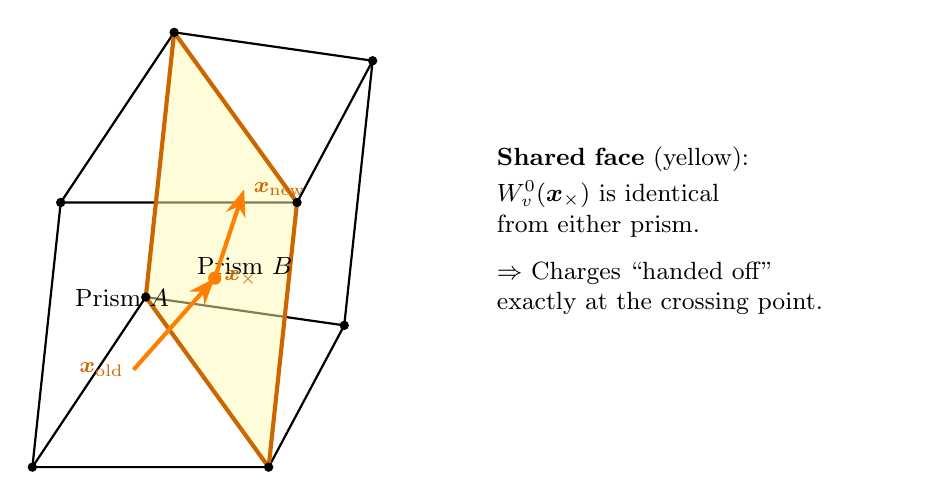
\begin{tikzpicture}[
    scale=1.2,
    >=Stealth,
    vert/.style={circle, fill=black, inner sep=1.2pt},
  ]
  % Prism A (left)
  \coordinate (A0) at (0, 0);
  \coordinate (B0) at (2.5, 0);
  \coordinate (C0) at (1.2, 1.8);
  \coordinate (A1) at ($(A0)+(0.3, 2.8)$);
  \coordinate (B1) at ($(B0)+(0.3, 2.8)$);
  \coordinate (C1) at ($(C0)+(0.3, 2.8)$);

  % Prism B (right, shares edge B-C)
  \coordinate (D0) at (3.3, 1.5);
  \coordinate (D1) at ($(D0)+(0.3, 2.8)$);

  % Draw prism A
  \draw[thick] (A0)--(B0)--(C0)--cycle;
  \draw[thick] (A1)--(B1)--(C1)--cycle;
  \draw[thick] (A0)--(A1) (B0)--(B1) (C0)--(C1);

  % Draw prism B
  \draw[thick] (B0)--(D0)--(C0);
  \draw[thick] (B1)--(D1)--(C1);
  \draw[thick] (D0)--(D1);

  % Shared face
  \fill[yellow!30, opacity=0.5] (B0)--(C0)--(C1)--(B1)--cycle;
  \draw[thick, orange!80!black, line width=1.5pt] (B0)--(C0) (B1)--(C1)
    (B0)--(B1) (C0)--(C1);

  % Vertices
  \foreach \p in {A0,B0,C0,D0,A1,B1,C1,D1} \node[vert] at (\p) {};

  % Labels
  \node[font=\small] at ($(A0)!0.33!(B0)!0.33!(C0)+(0,1.2)$) {Prism $A$};
  \node[font=\small] at ($(B0)!0.33!(D0)!0.33!(C0)+(0,1.2)$) {Prism $B$};

  % Trajectory
  \coordinate (Pold) at ($(A0)!0.4!(B0)!0.35!(C0)+(0,0.4)$);
  \coordinate (Pcross) at ($(B0)!0.5!(C0)+(0.08,1.1)$);
  \coordinate (Pnew) at ($(B0)!0.4!(D0)!0.45!(C0)+(0.15,1.8)$);

  \draw[->, thick, orange, line width=1.5pt] (Pold) -- (Pcross);
  \draw[->, thick, orange, line width=1.5pt] (Pcross) -- (Pnew);
  \fill[orange] (Pcross) circle (2pt);

  \node[font=\footnotesize, orange!80!black, left] at (Pold)
    {$\bm{x}_\text{old}$};
  \node[font=\footnotesize, orange!80!black, right] at (Pcross)
    {$\bm{x}_\times$};
  \node[font=\footnotesize, orange!80!black, right] at (Pnew)
    {$\bm{x}_\text{new}$};

  % Annotation
  \node[font=\small, text width=5cm, align=left] at (7.0, 2.5) {
    \textbf{Shared face} (yellow):\\[2pt]
    $W^0_v(\bm{x}_\times)$ is identical\\
    from either prism.\\[6pt]
    $\Rightarrow$ Charges ``handed off''\\
    exactly at the crossing point.
  };
\end{tikzpicture}
\caption{A particle crossing from prism $A$ to prism $B$ through a shared
  face (yellow). The trajectory is split at $\bm{x}_\times$, and the
  deposition formulas are applied independently in each prism. Charge
  conservation holds globally because the Whitney 0-forms are continuous
  across shared faces.}
\label{fig:multi_prism}
\end{figure}

When a particle crosses from prism $A$ to prism $B$
(Figure~\ref{fig:multi_prism}), the trajectory is split at the crossing point
$\bm{x}_\times$. Deposition is applied independently in each prism:
\begin{itemize}[nosep]
  \item In prism $A$: deposit from $\bm{x}_\text{old}$ to $\bm{x}_\times$.
  \item In prism $B$: deposit from $\bm{x}_\times$ to $\bm{x}_\text{new}$.
\end{itemize}

Charge conservation holds globally for three reasons:
\begin{enumerate}[nosep]
  \item \emph{Within each prism}: Theorem~\ref{thm:conservation} applies.
  \item \emph{Across shared faces}: $W^0_v$ is continuous, so the charge
    ``released'' by prism $A$ at $\bm{x}_\times$ exactly equals the charge
    ``received'' by prism $B$. For non-shared vertices,
    $W^0_v(\bm{x}_\times) = 0$.
  \item \emph{Total charge}: $\sum_v \rho_v = q$ by the partition of unity,
    independent of position.
\end{enumerate}

\paragraph{Detecting crossings.}
A particle exits a prism when any $\lambda_i < 0$ (angular crossing through a
rectangular face) or $\zeta \notin [0,1]$ (radial crossing through a
triangular face). The crossing point is found by linear interpolation. The new
prism is identified via the computable connectivity function.

%=============================================================================
\section{Field Interpolation}
\label{sec:interpolation}
%=============================================================================

To interpolate the electric field at a particle position $\bm{x}$ within a
prism, evaluate the Whitney 1-form expansion:
\begin{equation}
  \bm{E}(\bm{x}) = \sum_{e} \widetilde{E}_e\;W^1_e(\bm{x}),
\end{equation}
where the sum runs over the 9 edges of the containing prism. Each Whitney
1-form~\eqref{eq:W1h}--\eqref{eq:W1v} is a differential form that, when
evaluated in Cartesian components, yields a 3-vector at each point. The
evaluation requires only the barycentric coordinates $(\lambda_i)$ and the
radial parameter $\zeta$, plus the gradients $\nabla\lambda_i$ (which are
constant within a given triangle and precomputed at initialization).

Similarly, the magnetic field at a particle position is interpolated via the
2-form expansion using Whitney 2-forms~\eqref{eq:W2tri}--\eqref{eq:W2rect}.

%=============================================================================
% References
%=============================================================================
\begin{thebibliography}{99}

\bibitem{Tomita2002}
  H.~Tomita, M.~Tsugawa, M.~Satoh, and K.~Goto,
  ``Shallow water model on a modified icosahedral geodesic grid by using
  spring dynamics,''
  \emph{J.\ Comput.\ Phys.}, \textbf{174}, 579--613 (2001).

\bibitem{Pitassi2021}
  S.~Pitassi, R.~Trevisan, and R.~Specogna,
  ``Explicit geometric construction of sparse inverse mass matrices for
  arbitrary tetrahedral grids,''
  \emph{Comput.\ Methods Appl.\ Mech.\ Engrg.}, \textbf{377}, 113699 (2021).

\bibitem{DyczijEdlinger2006}
  R.~Dyczij-Edlinger and O.~Biro,
  ``Sparse and explicit FETD via approximate inverse Hodge (mass) matrix,''
  \emph{IEEE Trans.\ Magn.}, \textbf{42}(4), 1263--1266 (2006).

\bibitem{GEMPIC}
  M.~Kraus, K.~Kormann, P.~Morrison, and E.~Sonnendr\"ucker,
  ``GEMPIC: Geometric electromagnetic particle-in-cell methods,''
  \emph{J.\ Plasma Phys.}, \textbf{83}(4), 905830401 (2017).

\bibitem{Arnold2010}
  D.~N.~Arnold, R.~S.~Falk, and R.~Winther,
  ``Finite element exterior calculus: from Hodge theory to numerical
  stability,''
  \emph{Bull.\ Amer.\ Math.\ Soc.}, \textbf{47}(2), 281--354 (2010).

\bibitem{McRae2016}
  A.~T.~T.~McRae, G.-T.~Bercea, L.~Mitchell, D.~A.~Ham, and C.~J.~Cotter,
  ``Automated generation and symbolic manipulation of tensor product finite
  elements,''
  \emph{SIAM J.\ Sci.\ Comput.}, \textbf{38}(5), S25--S47 (2016).

\end{thebibliography}

\end{document}
